\documentclass[manuscript]{acmart}

\usepackage{tikz}
\usetikzlibrary{shapes.geometric, arrows.meta, positioning}
\usepackage{pgfplots}
\pgfplotsset{compat=1.18}
\usepackage{listings}
\usepackage{xcolor}
\usepackage{booktabs}
\usepackage{tcolorbox}
\usepackage{url}

% code listing style
\definecolor{kwblue}{RGB}{0,0,200}
\definecolor{listbg}{RGB}{245,245,250}

\lstdefinelanguage{Sollya}{
  morekeywords={prec,display,hexadecimal,decimal,rationalmode,off,
    guessdegree,remez,fpminimax,dirtyinfnorm,infnorm,supnorm,
    horner,canonical,round,evaluate,sup,inf,log2,log,exp,sin,cos,
    print,for,from,to,do,if,then,else,version,D,RN,relative,absolute},
  sensitive=true,
  morecomment=[l]{//},
  morestring=[b]",
}

\lstdefinestyle{sollya}{
  language=Sollya,
  backgroundcolor=\color{listbg},
  basicstyle=\ttfamily\small,
  keywordstyle=\color{kwblue},
  commentstyle=\color{gray},
  stringstyle=\color{kwblue},
  frame=single, framerule=0.4pt, rulecolor=\color{gray!50},
  numbers=none, breaklines=true, keepspaces=true,
}

\lstdefinestyle{cpp}{
  language=C++,
  backgroundcolor=\color{listbg},
  basicstyle=\ttfamily\small,
  keywordstyle=\color{kwblue},
  commentstyle=\color{gray},
  stringstyle=\color{gray!60!black},
  frame=single, framerule=0.4pt, rulecolor=\color{gray!50},
  numbers=none, breaklines=true, keepspaces=true,
}

\lstdefinestyle{shell}{
  language=bash,
  backgroundcolor=\color{listbg},
  basicstyle=\ttfamily\small,
  keywordstyle=\color{kwblue},
  commentstyle=\color{gray},
  frame=single, framerule=0.4pt, rulecolor=\color{gray!50},
  numbers=none, breaklines=true, keepspaces=true,
}

% TikZ styles for flow diagrams
\tikzstyle{flowbox} = [rectangle, rounded corners=2pt,
  fill=blue!12, draw=blue!40, minimum width=7cm, minimum height=0.9cm,
  align=center, font=\small]
\tikzstyle{decisionbox} = [diamond, aspect=2.5,
  fill=orange!15, draw=orange!60, minimum width=3.5cm, minimum height=1cm,
  align=center, font=\small]
\tikzstyle{arrow} = [-{Stealth}, thick]

% ACM metadata
\settopmatter{printacmref=false}
\renewcommand\footnotetextcopyrightpermission[1]{}

\title{Approximating Functions: A Practical Guide to Sollya and Function Implementation}
\author{CCMath}
\date{}

\begin{document}
\maketitle

% -----------------------------------------------------------------------
\section{The core problem}

A handful of operations are \emph{correctly rounded} on every conforming
platform: addition, subtraction, multiplication, division, square root, and
fused multiply-add are required by IEEE~754 to behave as if the exact result
were computed to infinite precision and rounded once~\cite{ieee}.
Almost everything else cannot be handled that way.

\texttt{exp}, \texttt{log}, \texttt{sin}, \texttt{cos}, \texttt{atan},
\texttt{pow}, \texttt{tgamma}, and the rest are transcendental or
algebraic-but-irrational.  There is no finite formula in terms of the basic
operations that yields their value exactly.

Implementing such a function is an engineering process with four recurring
stages~\cite{muller,handbook}:

\begin{enumerate}
\item \textbf{Argument reduction.}  Use mathematical identities to map
  the input into a small, well-behaved interval.
\item \textbf{Approximation.}  Replace the true function by a polynomial
  whose error is small and bounded by a proof.
\item \textbf{Reconstruction.}  Combine the approximation with information
  discarded during reduction to recover the full-range result.
\item \textbf{Rounding.}  Deliver the result correctly (or faithfully)
  rounded in the target format, in every rounding mode the function supports.
\end{enumerate}

Stages~1, 3, and~4 are function-specific algebra and careful
floating-point bookkeeping.  Stage~2 is where Sollya is used.

% -----------------------------------------------------------------------
\section{Polynomial approximation}

Polynomials are the natural tool.  They require only the four basic
operations, map well to hardware FMA, and their error can be bounded by
analysis.

Choosing coefficients so the error is small over an interval is the
approximation problem.  The wrong choice of norm or reference polynomial can
make the bound much worse than necessary.

% -----------------------------------------------------------------------
\section{Taylor approximation}

A Taylor series centered at zero has the form
\[
  f(x) = \sum_{k=0}^{\infty} \frac{f^{(k)}(0)}{k!}\, x^k.
\]
Truncating at degree $n$ gives a polynomial whose error is smallest at $x = 0$
and grows toward the interval edges.

\begin{figure}[h]
  \centering
  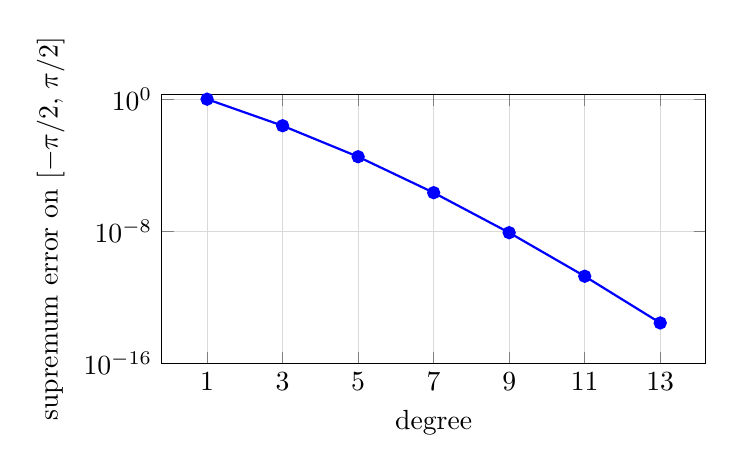
\begin{tikzpicture}
    \begin{semilogyaxis}[
      width=0.7\linewidth, height=5cm,
      xlabel={degree},
      ylabel={supremum error on $[-\pi/2,\,\pi/2]$},
      grid=both, grid style={gray!30},
      xtick={1,3,5,7,9,11,13},
      ymin=1e-16, ymax=2,
      mark size=2pt,
    ]
    \addplot[color=blue, mark=*, thick] coordinates {
      (1,  1.0)
      (3,  2.46e-2)
      (5,  3.26e-4)
      (7,  2.17e-6)
      (9,  8.22e-9)
      (11, 1.89e-11)
      (13, 2.81e-14)
    };
    \end{semilogyaxis}
  \end{tikzpicture}
  \caption{Supremum absolute error of odd Taylor sine polynomials on
  $[-\pi/2,\pi/2]$ as a function of degree.  Adding terms reduces the
  error, but the distribution is worst-case at the interval endpoints.}
\end{figure}

A Taylor polynomial can look excellent in a small hand test and still be
wrong for the interval.  The worst input on the interval controls the design.

For a fixed-degree polynomial in a fixed format, the usual choice is
minimax approximation.

% -----------------------------------------------------------------------
\section{Minimax approximation}

A minimax polynomial minimizes the largest error on an interval.

For many elementary functions, this is the right goal.  A minimax polynomial
spreads error across the interval instead of spending most of the accuracy
near one point.

For a degree $n$ polynomial, the best minimax approximation has an error
curve that reaches its maximum size at least $n + 2$ times, with alternating
signs~\cite{muller}.

The theorem gives a useful check.  If the error plot has one large spike and
many small regions, the polynomial is probably not close to minimax.  If the
peaks are balanced, the approximation is more likely to use the degree well.

Taylor approximation is local.  Minimax approximation is worst-case driven.

\begin{figure}[h]
  \centering
  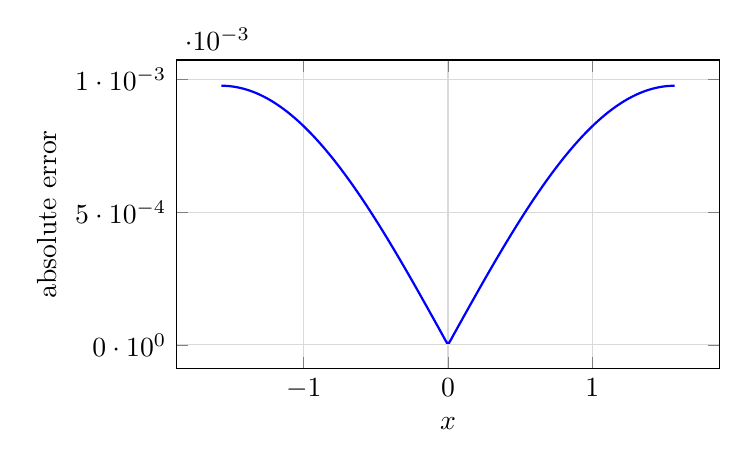
\begin{tikzpicture}
    \begin{axis}[
      width=0.7\linewidth, height=5.5cm,
      xlabel={$x$},
      ylabel={absolute error},
      grid=both, grid style={gray!30},
      yticklabel style={/pgf/number format/sci},
      ytick scale label code/.code={$\cdot 10^{-3}$},
      scaled y ticks={base 10:-3},
    ]
    \addplot[color=blue, thick, domain=-pi/2:pi/2, samples=200]
      { abs((x - x^3/6 + x^5/120) - sin(deg(x)*pi/180)) };
    \end{axis}
  \end{tikzpicture}
  \caption{Absolute error of the degree~5 Taylor approximation to
  $\sin(x)$ on $[-\pi/2,\pi/2]$.  The error is smallest near zero and
  grows toward the interval edges.}
\end{figure}

% -----------------------------------------------------------------------
\section{Remez}

The Remez exchange algorithm is the usual numerical method for computing a
minimax polynomial.

Remez repeatedly finds error peaks, adjusts the polynomial so that those
peaks are more evenly spaced, and then repeats until the error curve has the
minimax shape~\cite{muller}.

Sollya provides a \texttt{remez} command for this.

There is one important limit.  Remez gives a polynomial with real-number
coefficients.  Source code cannot store arbitrary real numbers.  It stores
\texttt{float}, \texttt{double}, \texttt{long}~\texttt{double},
fixed-width constants, or pairs such as double-double values.

A real-coefficient Remez polynomial is useful for exploration.  It is not
automatically the polynomial that belongs in the source code.

% -----------------------------------------------------------------------
\section{Coefficients must fit the machine}

If a real-coefficient minimax polynomial is rounded by hand, the result may
no longer have the minimax error shape.  The error can grow enough to break
the intended bound~\cite{muller}.

Sollya's \texttt{fpminimax} command addresses this problem.

\texttt{fpminimax} searches for a near-minimax polynomial whose coefficients
are already constrained to the requested formats~\cite{muller,handbook}.

Use the commands this way:

\begin{table}[h]
  \centering
  \begin{tabular}{ll}
    \toprule
    Step & Use \\
    \midrule
    \texttt{remez}    & Explore the real-coefficient approximation \\
    \texttt{fpminimax} & Generate coefficients for source code \\
    \bottomrule
  \end{tabular}
\end{table}

Do not hand-round production coefficients unless the rounded polynomial is
checked again.

A bad constant can ruin a good algorithm.  A decimal literal that looks
harmless may round differently than the value Sollya produced.  Prefer
hexadecimal constants when the value is meant to be exact in the target
format.

% -----------------------------------------------------------------------
\section{Absolute error and relative error}

Choose the error model before generating a polynomial.

Absolute error is:
\[ |p(x) - f(x)| \]

Relative error is:
\[ \left|\frac{p(x)}{f(x)} - 1\right| \]

Floating-point accuracy is often measured in ULPs.  ULP size changes with
the size of the result~\cite{handbook}.  Because of that, relative error is
often the right target.

Relative error is not always safe.  If $f(x)$ is close to zero, dividing by
$f(x)$ can make the relative error unstable.  Change the kernel.
Section~\ref{sec:kernel} lists the usual transformed kernels.

% -----------------------------------------------------------------------
\section{Sollya}

Sollya is the main approximation tool used in this workflow.

Use Sollya for these tasks:

\subsection{Running Sollya}

Run a script:
\begin{lstlisting}[style=shell]
sollya script.sollya
\end{lstlisting}

Start scripts like this:
\begin{lstlisting}[style=sollya]
prec = 200!;
display = hexadecimal!;
\end{lstlisting}

\begin{table}[h]
  \centering
  \caption{Sollya commands used in this guide.}
  \begin{tabular}{ll}
    \toprule
    Task & Sollya command \\
    \midrule
    Estimate the needed degree           & \texttt{guessdegree} \\
    Compute a real-coefficient minimax polynomial & \texttt{remez} \\
    Compute machine-format coefficients  & \texttt{fpminimax} \\
    Quickly estimate worst-case error    & \texttt{dirtyinfnorm} \\
    Compute a safer error bound          & \texttt{infnorm} or \texttt{supnorm} \\
    Print constants for source code      & \texttt{display = hexadecimal} \\
    Print Horner form                    & \texttt{horner} \\
    Print expanded form                  & \texttt{canonical} \\
    \bottomrule
  \end{tabular}
\end{table}

The precision setting controls Sollya's working precision.  It should be
higher than the target format.  For double coefficients, 200 bits is a
reasonable starting point.

Hexadecimal output matters.  It lets C++ store the same floating-point value
that Sollya printed.  Decimal constants can add another rounding step.

% -----------------------------------------------------------------------
\section{A small Sollya example}

Assume $\exp(x)$ has already been reduced to $\exp(r)$, where $r$ is close
to zero.

A common shape is:
\[ \exp(x) = 2^k \exp(r) \]
where $r$ lies in an interval such as:
\[ \left[-\frac{\log(2)}{2};\, \frac{\log(2)}{2}\right] \]

A first Sollya script:
\begin{lstlisting}[style=sollya]
prec = 200!;
display = hexadecimal!;

f = exp(x);
I = [-1/2 * log(2); 1/2 * log(2)];

guessdegree(f, I, 1b-53);

p = fpminimax(f, 6, [|D...|], I, relative);

eps_fast = dirtyinfnorm(p / f - 1, I);
print("approx relative error:", eps_fast, "bits:", log2(eps_fast));

supnorm(p, f, I, relative, 1b-40);
\end{lstlisting}

Read $\log_2(\text{error})$ as a rough number of correct bits.  If the error
is around $2^{-53}$, the approximation is near double precision.

This only bounds the polynomial approximation for $\exp(r)$ on the reduced
interval.  It does not prove \texttt{exp}.

The full function still needs reduction, floating-point evaluation,
reconstruction, special cases, and final rounding.

% -----------------------------------------------------------------------
\section{Choosing the kernel}
\label{sec:kernel}

The kernel is the smaller function approximated after reduction.

It is not always the public function.

For $\sin(x)$, the kernel may be $\sin(r)$.

For small $x$, it may be better to approximate $\sin(r)$ divided by $r$.

For $\log1\mathrm{p}(x)$, it may be better to approximate $\log(1+r)$
divided by $r$.

For $\mathrm{expm1}(x)$, it may be better to approximate
$\mathrm{expm1}(r)$ divided by $r$.

The choice matters.  A good kernel removes cancellation, avoids bad relative
error near zero, and reduces the polynomial degree.

Use the algebra of the function before asking Sollya for coefficients.

What should be small after reduction, and what should be exact?  That choice
often determines the kernel.

\subsection{Small-input transforms}
\begin{align*}
  \log(1+x) &= x \cdot \frac{\log(1+x)}{x} \\[4pt]
  \exp(x)-1  &= x \cdot \frac{\exp(x)-1}{x} \\[4pt]
  \sin(x)    &= x \cdot \frac{\sin(x)}{x} \\[4pt]
  \cos(x)    &= 1 - 2\sin^2\!\left(\tfrac{x}{2}\right)
\end{align*}

These forms are useful near zero.  They factor out the part that causes
cancellation or bad relative error.  The implementation approximates the
smoother quotient or uses a reconstruction identity that keeps more useful
bits.

The identity must still be checked on the target interval and under the
target rounding policy.  None of these forms is automatically best on every
interval.

% -----------------------------------------------------------------------
\section{Worked example: a small sine kernel}

\begin{tcolorbox}[colback=blue!5, colframe=blue!30, title={Start here for hands-on work}]
If you want to run Sollya and follow code in order, begin with
Section~\ref{sec:setup} and Section~\ref{sec:target}.
Skim Sections~1--7 first if the approximation vocabulary is new.
\end{tcolorbox}

\vspace{0.5em}

This example implements a restricted function:
\[
  \texttt{sin\_small}(x) \approx \sin(x) \quad \text{for } |x| \le \tfrac{1}{16}
\]

It is not a full implementation of \texttt{sin}.  It has no quadrant logic,
no large-input reduction, and no special-case table.  The whole kernel fits
on one screen.

\subsection{Set up Sollya}
\label{sec:setup}

The worked examples need Sollya only.  Install it once, then run the scripts
under \texttt{sollya/} from this guide directory:

\begin{lstlisting}[style=shell]
# macOS
brew install sollya

# Debian/Ubuntu
sudo apt install sollya

sollya sollya/sin_small_error.sollya
\end{lstlisting}

The build script runs the same scripts when you rebuild the guide PDF\@.
MPFR, Gappa, Rocq, and SageMath are useful later for validation, but they
are not required to follow the examples here.

\subsection{Specify the target}
\label{sec:target}

\begin{center}
\begin{tabular}{ll}
  Target: & $f(x) = \sin(x)$ \\[3pt]
  Input interval: & $x \in \left[-\dfrac{1}{16},\, \dfrac{1}{16}\right]$ \\[8pt]
  Output type: & \texttt{double} \\[3pt]
  Accuracy target for this example: & well below 1~ULP on the stated interval under round-to-nearest \\
\end{tabular}
\end{center}

This example is only a teaching kernel.  A full CCMath function would also
need all standard special cases and all supported rounding modes.

\subsection{Choose the kernel}

Directly approximating $\sin(x)$ works on this interval, but the odd symmetry
is useful.  Since $\sin(x)$ is odd:
\[
  \sin(x) = x q(x^2)
\]
where:
\[
  q(z) = \frac{\sin(\sqrt{z})}{\sqrt{z}}
\]

Near zero, $q(z)$ is smooth and close to~1.

The implementation will compute:
\[
  z = x^2
\]
and:
\[
  \sin(x) \approx x\,p(z)
\]
where $p$ approximates $q$.

\subsection{Pick a simple polynomial}

For a teaching example, the Taylor terms are easy to inspect:
\[
  \sin(x) = x - \frac{x^3}{6} + \frac{x^5}{120} - \frac{x^7}{5040} +
             \frac{x^9}{362880} + \cdots
\]

Factoring out $x$ gives:
\[
  \sin(x) = x\!\left(1 - \frac{z}{6} + \frac{z^2}{120} - \frac{z^3}{5040} +
            \frac{z^4}{362880} + \cdots\right)
\]
where $z = x^2$.

For production work, use \texttt{fpminimax} and record the bound.  Here, the
Taylor coefficients keep the example readable, and Sollya is used to check the
error.

\subsection{Check the approximation in Sollya}

Use Sollya to bound the error over the actual interval:
\begin{lstlisting}[style=sollya]
prec = 200!;
display = hexadecimal!;

I = [-1/16; 1/16];

p = x * (
    0x1.0000000000000p+0
  + x^2 * (
      -0x1.5555555555555p-3
    + x^2 * (
        0x1.1111111111111p-7
      + x^2 * (
          -0x1.a01a01a01a01ap-13
        + x^2 * 0x1.71de3a556c734p-19
      )
    )
  )
);

abs_err = supnorm(p, sin(x), I, absolute, 1b-80);
rel_err = supnorm(p, sin(x), I, relative, 1b-80);

print("absolute error:", abs_err);
print("relative error:", rel_err);
\end{lstlisting}

The code is not accepted because the series looks familiar.  It is accepted
only after the interval and error are checked.

\subsection{Implement the kernel}

A compact C++ implementation can use Horner form:
\begin{lstlisting}[style=cpp]
[[nodiscard]] constexpr double sin_small(double x) noexcept
{
    const double z = x * x;

    const double p =
        (((0x1.71de3a556c734p-19 * z
         - 0x1.a01a01a01a01ap-13) * z
         + 0x1.1111111111111p-7) * z
         - 0x1.5555555555555p-3) * z
         + 0x1.0000000000000p+0;

    return x * p;
}
\end{lstlisting}

There is no range check in this kernel.  The caller is responsible for
sending only values in the promised interval.  In a real internal
implementation, that precondition should be enforced by the surrounding
reduction path or by tests that call the kernel only on the reduced interval.

\subsection{Test the kernel}

For this restricted kernel, useful tests include:

\begin{enumerate}
\item $x$ equals~$0$
\item $x$ equals the interval endpoints
\item several values near the endpoints
\item positive and negative inputs with matching signs
\item comparison against MPFR or another high-precision oracle
\end{enumerate}

A simple round-to-nearest test should compare the returned bit pattern or ULP
distance, not printed decimal text.

Example values:
\[
  0,\quad \frac{1}{1024},\quad -\frac{1}{1024},\quad \frac{1}{32},\quad
  -\frac{1}{32},\quad \frac{1}{16},\quad -\frac{1}{16}
\]

The endpoints matter because the approximation was proved only on that
interval.  If a later change expands the interval to $[-1/8,1/8]$, the proof
and tests must be redone.

\begin{figure}[h]
  \centering
  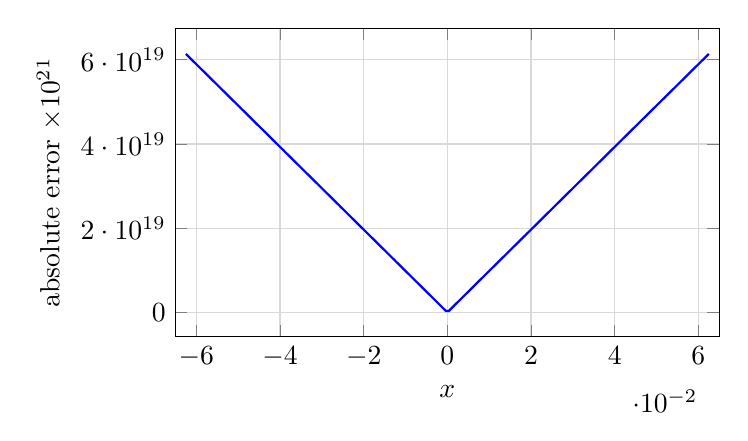
\begin{tikzpicture}
    \begin{axis}[
      width=0.7\linewidth, height=5.5cm,
      xlabel={$x$},
      ylabel={absolute error $\times 10^{21}$},
      grid=both, grid style={gray!30},
      xmin=-0.065, xmax=0.065,
      scaled y ticks=false,
      ytick scale label code/.code={},
    ]
    \addplot[color=blue, thick, domain=-0.0625:0.0625, samples=200]{
      abs((x * (1 + x*x*(-1/6 + x*x*(1/120 + x*x*(-1/5040 + x*x/362880))))
           - sin(deg(x)*pi/180))) * 1e21
    };
    \end{axis}
  \end{tikzpicture}
  \caption{Scaled absolute error of the small sine teaching polynomial on
  $[-1/16,1/16]$.  The plot shows the approximation error for the restricted
  kernel, not the error of a full \texttt{sin} implementation.}
\end{figure}

\subsection{What this example leaves out}

This small kernel does not implement full \texttt{sin}.

A full implementation still needs:

\begin{enumerate}
\item reduction for arbitrary finite inputs
\item quadrant reconstruction
\item handling of NaN and infinities
\item signed-zero behavior
\item directed rounding behavior
\item large-input Payne-Hanek reduction
\item validation against an oracle
\item a recorded error budget for reduction, evaluation, and reconstruction
\end{enumerate}

The subsections above follow the same loop used inside larger functions.
The larger versions add reduction, tables, multiple precision tiers, special
cases, and harder rounding decisions.

% -----------------------------------------------------------------------
\section{Advanced worked example: a small log2 core}
\label{sec:log2}

This example shows a more advanced shape than the small sine kernel.  It uses
a table reduction, a transformed kernel, split constants, and a polynomial on
a small residual interval.

The goal is not to implement full $\log_2$.  The example implements the core
used after the input has already been decomposed as:
\[ x = m 2^e \]
with:
\[ m \in [1, 2) \]

The full result is:
\[ \log_2(x) = e + \log_2(m) \]

The core computes the $\log_2(m)$ part.

\subsection{Choose the table reduction}

Divide $[1, 2)$ into $B$ buckets.  For a teaching version, use:
\[ B = 16 \]

For each bucket, choose a value $r_i$ close to the reciprocal of the bucket
center.  For an input mantissa $m$, compute:
\[ u = m r_i - 1 \]

If $r_i$ is well chosen, $u$ is small.  The identity is:
\[ m = \frac{1 + u}{r_i} \]
so:
\[ \log_2(m) = \log_2(1 + u) - \log_2(r_i) \]

The table stores $r_i$ and a split form of $-\log_2(r_i)$.

One split is:
\[ -\log_2(r_i) = h_i + \ell_i \]

The high part $h_i$ can be rounded to fewer bits so that adding it to the
exponent is exact in the fast path.  The low part $\ell_i$ carries the
remaining bits.

\subsection{What the table buys}

The table makes the polynomial interval smaller.  With $B = 16$, a simple
bucket-center choice gives a residual roughly bounded by:
\[ |u| \le \frac{1}{2B} \]

The exact bound depends on how the buckets and reciprocals are chosen.  The
point is that more table bits shrink the interval that the polynomial has to
cover.

This is the usual tradeoff.  A larger table costs memory and cache pressure.
A smaller residual can reduce polynomial degree or make the error proof easier.

\subsection{Approximate the residual function}

After the table reduction, the remaining function is:
\[ \log_2(1 + u) \]

Since $u$ is small, approximate:
\[ g(u) = \frac{\log_2(1 + u)}{u} \]

Then:
\[ \log_2(1 + u) \approx u\,p(u) \]

This avoids a zero at $u = 0$.  The function $g(u)$ is smooth near zero,
with value $1/\log(2)$.

A Sollya script for the polynomial looks like this:
\begin{lstlisting}[style=sollya]
prec = 200!;
display = hexadecimal!;

U = [-1/32; 1/32];
g = log2(1 + x) / x;

p = fpminimax(g, 5, [|D...|], U, relative);

abs_err = supnorm(x * p, log2(1 + x), U, absolute, 1b-80);
rel_err = supnorm(p, g, U, relative, 1b-80);

print("absolute residual error:", abs_err);
print("relative kernel error:", rel_err);
print("polynomial:");
horner(p);
\end{lstlisting}

This checks the part controlled by the polynomial.  It does not check table
indexing, the split constants, or the final addition with the exponent.

\begin{figure}[h]
  \centering
  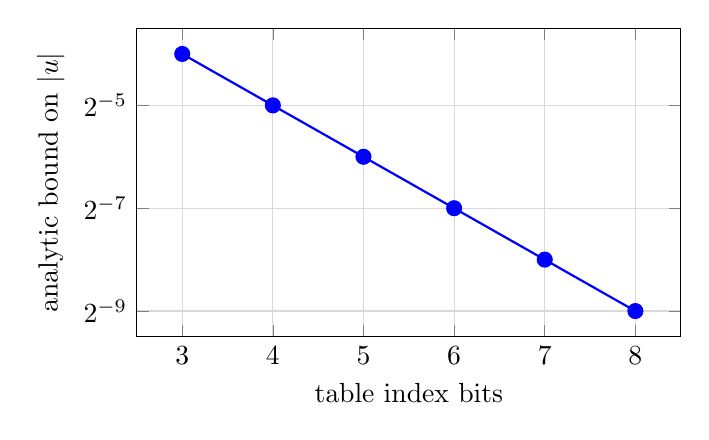
\begin{tikzpicture}
    \begin{axis}[
      width=0.7\linewidth, height=5.5cm,
      xlabel={table index bits},
      ylabel={analytic bound on $|u|$},
      ymode=log, log basis y=2,
      grid=both, grid style={gray!30},
      xtick={3,4,5,6,7,8},
      mark size=2.5pt,
    ]
    \addplot[color=blue, mark=*, thick] coordinates {
      (3, 0.0625)
      (4, 0.03125)
      (5, 0.015625)
      (6, 0.0078125)
      (7, 0.00390625)
      (8, 0.001953125)
    };
    \end{axis}
  \end{tikzpicture}
  \caption{Analytic residual bound after one reciprocal table reduction.
  More table bits shrink the interval used by the polynomial.}
\end{figure}

\subsection{Generate the table}

The table should be generated from the invariant, not typed by hand.

For each bucket, generate:
\begin{align*}
  c_i &= 1 + \frac{i + 1/2}{B} \\
  r_i &= \mathrm{round}_D\!\left(\frac{1}{c_i}\right) \\
  a_i &= -\log_2(r_i)
\end{align*}

Then split $a_i$ into a high part and a low part:
\begin{align*}
  h_i &= \mathrm{round}_t(a_i) \\
  \ell_i &= \mathrm{round}_D(a_i - h_i)
\end{align*}

Here $t$ is the chosen precision for the high part.  It should be chosen so
that the later addition with the exponent is exact for the path being proved.

A Sollya table script can be shaped like this:
\begin{lstlisting}[style=sollya]
prec = 200!;
display = hexadecimal!;

B = 16!;
hi_bits = 32!;

for i from 0 to B - 1 do {
  c = 1 + (i + 0.5) / B;
  r = round(1 / c, D, RN);
  a = -log2(r);
  hi = round(a, hi_bits, RN);
  lo = round(a - hi, D, RN);
  print("{", r, ", ", hi, ", ", lo, "},");
};
\end{lstlisting}

The generated log should record $B$, \texttt{hi\_bits}, the residual
interval, and the Sollya version.

\subsection{Kernel shape}

The implementation should make the data flow visible.  The following code
shows the shape without embedding generated table values in the guide:

\begin{lstlisting}[style=cpp]
struct Log2TableEntry
{
    double r;
    double hi;
    double lo;
};

struct Log2Poly
{
    double c1;
    double c2;
    double c3;
    double c4;
    double c5;
};

[[nodiscard]] constexpr double log2_core_small(double m,
                                               int e,
                                               const Log2TableEntry* table,
                                               const Log2Poly coeff) noexcept
{
    const int i = static_cast<int>((m - 1.0) * 16.0);
    const Log2TableEntry entry = table[i];

    const double u = std::fma(m, entry.r, -1.0);
\end{lstlisting}

\begin{figure}[h]
  \centering
  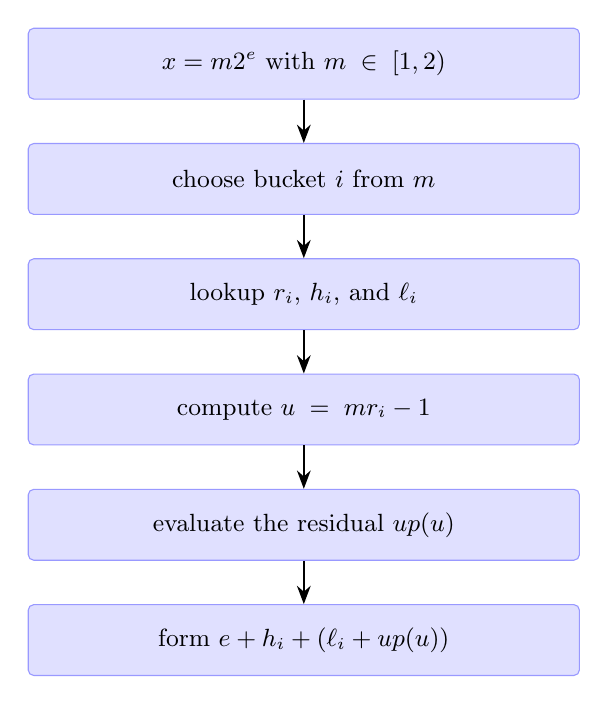
\begin{tikzpicture}[node distance=0.55cm]
    \node (input)  [flowbox] {$x = m2^e$ with $m \;\in\; [1, 2)$};
    \node (bucket) [flowbox, below=of input]  {choose bucket $i$ from $m$};
    \node (lookup) [flowbox, below=of bucket] {lookup $r_i$, $h_i$, and $\ell_i$};
    \node (compu)  [flowbox, below=of lookup] {compute $u \;=\; mr_i - 1$};
    \node (eval)   [flowbox, below=of compu]  {evaluate the residual $up(u)$};
    \node (form)   [flowbox, below=of eval]   {form $e + h_i + (\ell_i + up(u))$};

    \draw[arrow] (input)  -- (bucket);
    \draw[arrow] (bucket) -- (lookup);
    \draw[arrow] (lookup) -- (compu);
    \draw[arrow] (compu)  -- (eval);
    \draw[arrow] (eval)   -- (form);
  \end{tikzpicture}
  \caption{Data flow in the small $\log_2$ core.}
\end{figure}

\begin{lstlisting}[style=cpp]
    const double p =
        (((coeff.c5 * u + coeff.c4) * u + coeff.c3) * u + coeff.c2) * u
        + coeff.c1;

    const double residual = u * p;
    const double tail = entry.lo + residual;

    return (static_cast<double>(e) + entry.hi) + tail;
}
\end{lstlisting}

The coefficient object is produced from the Sollya polynomial.  The table
object is produced by the table-generation script.  Production code should
store those generated values directly in the implementation or in the nearby
generated constants file.

\subsection{What must be proved}

This example has more moving parts than the small sine kernel.  The proof
needs bounds for:

\begin{enumerate}
\item table index selection
\item reciprocal-table rounding
\item the size of $u$
\item the polynomial approximation to $\log_2(1 + u)$
\item the floating-point evaluation of $u\,p(u)$
\item the split addition $e + h_i + \ell_i$
\item the final rounding under each supported mode
\end{enumerate}

A Gappa proof is a good fit for the straight-line part after the table entry
has been chosen.  MPFR testing should cover bucket boundaries, values where
$u$ is near its largest magnitude, exact powers of two, subnormals routed
through the full log path, and every supported rounding mode.

\subsection{What this example leaves out}

This is not a complete $\log_2$ implementation.

A full function still needs:

\begin{enumerate}
\item bit decomposition for all finite positive inputs
\item handling of zero, negative inputs, NaN, and infinities
\item subnormal normalization
\item a larger or more carefully designed table
\item directed rounding checks
\item an accurate path for hard cases if correct rounding is the target
\end{enumerate}

The example shows the shape used by real kernels: reduce with a table, keep
the residual small, approximate a smooth transformed function, split constants
for exactness, and prove the operation sequence that is actually compiled.

% -----------------------------------------------------------------------
\section{The sign, exponent, and significand split}

A normal finite binary floating-point number can be written as~\cite{ieee,handbook}:
\[ x = s_x \cdot 2^{e_x} \cdot (1 + m_x) \]

This decomposition applies to finite nonzero normal binary floating-point
numbers.

\begin{itemize}
\item $s_x$ is the sign, either $+1$ or $-1$
\item $e_x$ is the unbiased binary exponent
\item $m_x$ is the fractional part of the significand
\item $1 + m_x$ is the normalized significand and lies in $[1, 2)$
\end{itemize}

For example:
\[ 6.5 = 1.625 \cdot 2^2 \]
so:
\begin{align*}
  s_x &= +1 \\
  e_x &= 2 \\
  m_x &= 0.625 \\
  6.5 &= +1 \cdot 2^2 \cdot (1 + 0.625)
\end{align*}

In binary:
\[ 6.5 = 110.1_2 = 1.101_2 \cdot 2^2 \]

The exponent carries scale.  The significand stays in a fixed interval.
This turns a problem over many magnitudes into a smaller approximation
problem plus exponent bookkeeping.

The $(1 + m_x)$ form is for normal numbers.  Subnormal numbers do not have
the implicit leading~1 and need normalization or special handling.  Zero,
infinity, and NaN do not fit this decomposition~\cite{ieee}.  Negative bases
for \texttt{pow} need integer-exponent handling before any logarithmic path.

% -----------------------------------------------------------------------
\section{Argument reduction}

Approximation works well only on a small interval.  Argument reduction is
how the implementation gets there~\cite{muller,handbook}.

For \texttt{exp}:
\[ \exp(x) = 2^k \exp(r) \]
where:
\[ k \approx \mathrm{round}\!\left(\frac{x}{\log(2)}\right) \]
and:
\[ r = x - k\log(2) \]

The integer $k$ carries the power-of-two scale.  The residual $r$ is small
enough for a short polynomial.

For $\exp_2$, the split is simpler:
\[ 2^x = 2^k 2^r \]
where:
\[ k = \lfloor x \rfloor \]
and:
\[ r = x - k \]

The reconstruction step puts $2^k$ back into the exponent field when the
result is in range.

For $\log_2$, the sign, exponent, and significand split gives:
\[ \log_2(x) = e_x + \log_2(1 + m_x) \]

For natural log:
\[ \log(x) = e_x \log(2) + \log(1 + m_x) \]

The exponent term is exact integer bookkeeping.  The hard part is
approximating the significand term, where $(1 + m_x)$ lies in a fixed
interval for normal inputs.

This is why log implementations usually extract the exponent first, reduce
the significand, and approximate only a small residual.

For trig functions, the usual reduction is modulo $\pi/2$ or $\pi/4$,
followed by quadrant reconstruction.

Trig reduction is hard for large inputs.  $\pi$ is irrational.  If $x$ is
huge and close to a multiple of $\pi/2$, subtracting $k\pi/2$ can lose the
useful bits.

\subsection{Cody-Waite reduction}

Cody-Waite reduction stores the reduction constant as a sum of machine
numbers:
\[ C = C_\mathrm{hi} + C_\mathrm{mid} + C_\mathrm{lo} \]
\[ r = x - kC_\mathrm{hi} - kC_\mathrm{mid} - kC_\mathrm{lo} \]

The split lets the subtraction keep more useful bits than one rounded
constant would keep.  The exact split depends on the function, interval, and
target precision.

\subsection{Payne-Hanek reduction}

Payne-Hanek reduction uses many precomputed bits of the reduction constant
and a higher-precision multiplication~\cite{muller}.

This is the large-input path for trig functions.  Ordinary double arithmetic
is not enough to reduce every double modulo $\pi/2$.

\begin{figure}[h]
  \centering
  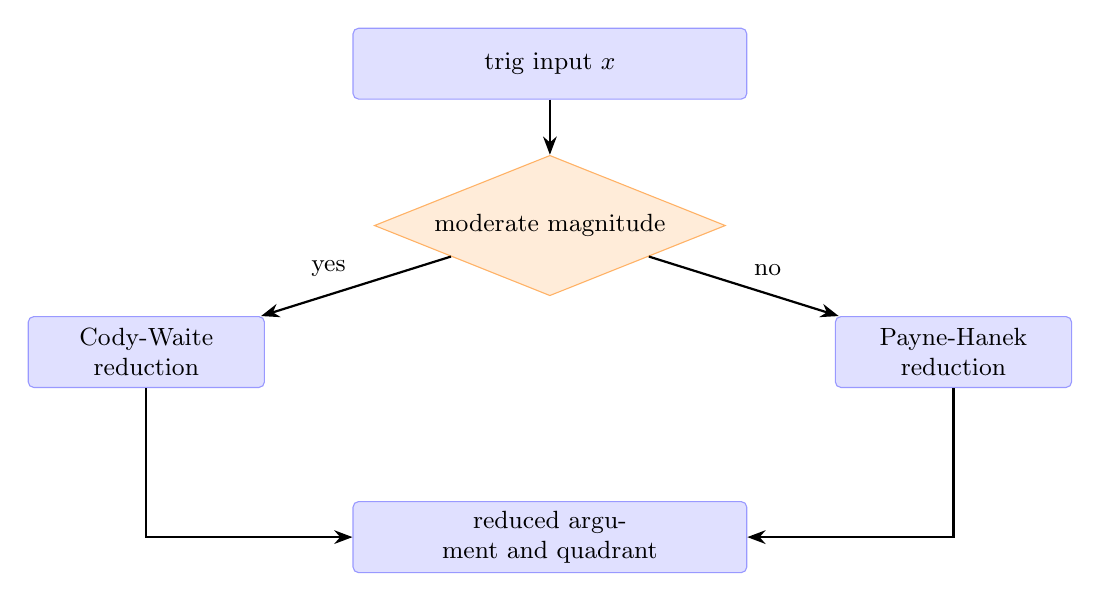
\begin{tikzpicture}[node distance=0.7cm and 2.5cm]
    \node (inp)  [flowbox, minimum width=5cm] {trig input $x$};
    \node (dec)  [decisionbox, below=of inp]      {moderate magnitude};
    \node (cw)   [flowbox, minimum width=3cm, below left=of dec]  {Cody-Waite\\reduction};
    \node (ph)   [flowbox, minimum width=3cm, below right=of dec] {Payne-Hanek\\reduction};
    \node (out)  [flowbox, minimum width=5cm, below=2.6cm of dec] {reduced argu-\\ment and quadrant};

    \draw[arrow] (inp) -- (dec);
    \draw[arrow] (dec) -- node[above left,  font=\small]{yes} (cw);
    \draw[arrow] (dec) -- node[above right, font=\small]{no}  (ph);
    \draw[arrow] (cw)  |- (out);
    \draw[arrow] (ph)  |- (out);
  \end{tikzpicture}
  \caption{Typical trig reduction split between moderate and large inputs.}
\end{figure}

\subsection{Trig quadrant reconstruction}

\[ x = k\frac{\pi}{2} + r \]

The reducer chooses an integer $k$ and a small residual $r$.  The value of
$k \bmod 4$ decides which small kernel reconstructs the result~\cite{muller}.

\begin{table}[h]
  \centering
  \begin{tabular}{cl}
    \toprule
    $k \bmod 4$ & $\sin(x)$ reconstruction \\
    \midrule
    0 & $\sin(r)$ \\
    1 & $\cos(r)$ \\
    2 & $-\sin(r)$ \\
    3 & $-\cos(r)$ \\
    \bottomrule
  \end{tabular}
\end{table}

This is why a full trig function is not just one polynomial.  The reducer
and quadrant logic decide which kernel is used and which sign is returned.

\subsection{Reduction error}

Reduction has its own error.

If the polynomial was proved for an exact reduced argument $r$, but the
implementation computes $r$ with too much error, the proof no longer applies.

Decide the total error target first.  Give part of that budget to reduction.
The reducer should carry enough extra precision that its error stays below
that budget.

For many functions, this means split constants or a double-word reduced
argument.  For very large trig inputs, it can mean a separate large-argument
reducer.

% -----------------------------------------------------------------------
\section{Evaluating the polynomial}

After Sollya gives coefficients, the implementation still has to evaluate
the polynomial in floating point.

The mathematical polynomial and the C++ expression are not identical.  Every
floating-point operation can round.

\subsection{Horner evaluation}

Horner evaluation is the usual default:
\[ p(x) = c_0 + x(c_1 + x(c_2 + x(\cdots))) \]

It uses few operations and maps well to FMA~\cite{muller,handbook}.

With FMA, one step can be:
\begin{lstlisting}[style=cpp]
r = fma(r, x, c);
\end{lstlisting}

That rounds the multiply-add once.

\subsection{Estrin evaluation}

Estrin evaluation groups terms so more work can happen in
parallel~\cite{handbook}.

For example:
\[ c_0 + c_1 x + c_2 x^2 + c_3 x^3 \]
can be grouped as:
\[ (c_0 + c_1 x) + x^2(c_2 + c_3 x) \]

This can be faster on wide cores.  It can also need more temporaries.  Use it
when measurements show that it helps.

\subsection{Double-word evaluation}

Some kernels need more precision in part of the evaluation.

Common tools include Fast2Sum, 2Sum, 2MultFMA, Veltkamp-Dekker splitting,
double-double arithmetic, and compensated Horner evaluation~\cite{muller,handbook}.

Do not use double-double everywhere by default.  Use it where the error
budget needs it.

The most useful extra precision is usually local.  It protects one reduction,
one product, or one reconstruction step.  Treat it as a tool for a specific
bound, not as a blanket fix.

% -----------------------------------------------------------------------
\section{Fast precision and accurate precision}

Many elementary functions use more than one precision tier.

The fast path should be cheap.  It handles ordinary inputs where a modest
amount of extra precision is enough.  The accurate path handles cases where
the result is too close to a rounding boundary, or where the fast path cannot
prove the final rounding decision.

For float functions, the implementation can often use double or double-double
arithmetic for the fast path.  Some cases may need a wider accurate path.

For double functions, the fast path usually needs a double-double-like
computation.  That does not mean every operation should behave like a complete
higher-precision type.  A full double-double type that renormalizes after
every operation is often too expensive for the hot path.

A faster pattern is to arrange the computation so that important intermediate
pieces are exact, or have a known error, and normalize only where the bound
needs it.  This is less general than a full double-double type, but it fits a
fixed numerical kernel better.

The accurate path may use a dyadic floating-point type with a fixed integer
significand, such as a 128-bit or 256-bit dyadic format.  This gives a large
exponent range and controlled precision without relying on hardware quad
precision.

Quad precision and double-double are not interchangeable.

Quad precision has a much larger exponent range than double-double.  A pair
of doubles gives extra significand bits, but it does not cheaply give the
exponent range of a true quad format.  A dyadic format can be a better
accurate-path type when the algorithm needs wide range and predictable fixed
precision.

One tiering pattern is:

\begin{table}[h]
  \centering
  \begin{tabular}{ll}
    \toprule
    Tier & Role \\
    \midrule
    double or double-double-like & Fast path \\
    128-bit dyadic & First accurate path \\
    256-bit dyadic & Hard-case path when needed \\
    \bottomrule
  \end{tabular}
\end{table}

This is especially relevant for \texttt{pow}.  A double \texttt{pow}
implementation is harder than a float \texttt{pow} implementation because the
final result has a 53-bit significand.  The intermediate log, multiply, and
exp reconstruction must leave enough margin for correct rounding.

% -----------------------------------------------------------------------
\section{Lookup tables}

Lookup tables in elementary functions are not only cached constants.

A table entry usually exists to make one reduction step cheaper, more
accurate, or both.  For log and pow, common table values include
approximations to quantities like $-\log_2(r)$, split into pieces.

A split table might store:
\[ a = -\log_2(r) \]
and:
\[ a = a_\mathrm{hi} + a_\mathrm{mid} + a_\mathrm{lo} \]

The split is chosen for a reason.  A high part may be rounded to a smaller
precision so that a later multiplication is exact, or so that adding it to
an exponent does not lose important bits.

Table generation should start from an invariant, not from a literal list of
constants.

A table-generation note should record:

\begin{enumerate}
\item how the index is chosen
\item what real value each entry approximates
\item how the entry is split
\item which later operation is meant to be exact or tightly bounded
\item what interval remains after the table reduction
\item which precision tier uses the table
\end{enumerate}

For \texttt{powf}, the fast path may use tables split into double-double or
triple-double pieces because the target result is float.  For \texttt{pow} in
double, the accurate paths may need tables generated directly for the wider
dyadic type used in that path.

Do not assume one table layout fits every precision tier.

If the accurate pass uses a 128-bit dyadic format, generate a table suited to
that format.  If there is a 256-bit hard-case path, generate the table for
that path as well.  The values may represent the same mathematical constants,
but the split, precision, and exactness constraints can be different.

A table without its generation rule is hard to audit.  A table with its
invariant is part of the proof.

\subsection{Log table reduction}

\[ \log_2(1 + m_x) = -\log_2(r_i) + \log_2(r_i(1 + m_x)) \]

Define:
\[ u = r_i(1 + m_x) - 1 \]

Then:
\[ \log_2(1 + m_x) = -\log_2(r_i) + \log_2(1 + u) \]

The table value $r_i$ is chosen so that $u$ is small.  The polynomial only
approximates $\log_2(1 + u)$ on a smaller interval.  The table entry supplies
the correction term $-\log_2(r_i)$.

This is the value of the table.  It is not only avoiding a computation.  It
makes the residual small enough for a cheaper and more accurate polynomial.
Section~\ref{sec:log2} uses the same pattern with bucket reciprocals and
split $-\log_2(r_i)$ constants.

% -----------------------------------------------------------------------
\section{Why pow is harder than exp or log}

\texttt{pow} combines the difficulties of log and exp.

For positive finite $x$, the usual shape is:
\begin{align*}
  \mathrm{pow}(x, y) &= \exp(y \log(x)) \\
  \mathrm{pow}(x, y) &= 2^{y \log_2(x)}
\end{align*}

\[ y \log_2(x) = y(e_x + \log_2(1 + m_x)) \]

This is why pow implementations often contain a log core, table reduction for
the significand, split constants, and extra precision around the product
$y \log_2(x)$.  A small error in the log value can be magnified by $y$, then
carried into the exp reconstruction.

That hides several problems.

First, $\log(x)$ needs its own range reduction, tables, approximation, and
reconstruction.

Second, $y \log(x)$ can magnify error.  If $y$ is large, a small log error
can become a large exponent error.

Third, \texttt{exp} has to reconstruct the final result, including overflow
and underflow behavior.

Fourth, \texttt{pow} has many special cases.  Negative bases, integer
exponents, zeros, infinities, NaNs, signed zeros, odd and even integer
exponents, and directed rounding modes all matter.

Because of this, \texttt{pow} is not a good first elementary function.

A better path is:

\begin{enumerate}
\item implement one exp-family function
\item implement one log-family function
\item learn the reduction, table, polynomial, and rounding structure
\item then implement pow
\end{enumerate}

\texttt{pow} is best understood as a composition of those two families, plus
a large special-case layer and a harder final-rounding problem.

% -----------------------------------------------------------------------
\section{Compiler behavior}

An error proof assumes a specific sequence of floating-point operations.  The
compiler may change that sequence unless the source and build settings prevent
it.

The main hazards are:

\begin{table}[h]
  \centering
  \begin{tabular}{ll}
    \toprule
    Hazard & Why it matters \\
    \midrule
    FMA contraction & \texttt{a*b + c} may become one fused operation \\
    Reassociation   & fast-math may reorder arithmetic \\
    Default rounding assumptions & directed modes may be ignored \\
    Hidden precision & intermediates may have different width \\
    Floating-point environment access & \texttt{fenv} support differs by compiler \\
    \bottomrule
  \end{tabular}
\end{table}

These two expressions do not have the same rounding behavior:
\begin{lstlisting}[style=cpp]
a * b + c
\end{lstlisting}
\begin{lstlisting}[style=cpp]
std::fma(a, b, c)
\end{lstlisting}

The first can round the product and then the sum.  The second rounds once.

If a proof needs FMA, use FMA explicitly.  If a proof needs the live rounding
mode, compile in a mode that respects it.  Do not prove one operation sequence
and compile a different one~\cite{handbook}.

This also affects double-double arithmetic.  Some exact multiplication
algorithms for double-double arithmetic without FMA are only valid under
round-to-nearest.  Making them correct under directed rounding can require
extra handling.  That cost belongs in the design.

% -----------------------------------------------------------------------
\section{The error budget}

\[
  E_\mathrm{total} \le E_\mathrm{reduce} + E_\mathrm{approx} +
  E_\mathrm{eval} + E_\mathrm{reconstruct} + E_\mathrm{round}
\]

\begin{itemize}
\item $E_\mathrm{reduce}$ comes from argument reduction
\item $E_\mathrm{approx}$ comes from replacing the function with a
  polynomial or rational function
\item $E_\mathrm{eval}$ comes from evaluating that approximation in
  floating point
\item $E_\mathrm{reconstruct}$ comes from scaling, sign changes, table
  corrections, and final algebra
\item $E_\mathrm{round}$ is the margin needed for the final rounding
  decision
\end{itemize}

This inequality is a model for thinking about the implementation.  It is not
always the final tight proof.  It is useful because it prevents a common
mistake: proving the polynomial and forgetting the rest of the function.

% -----------------------------------------------------------------------
\section{Correct rounding}

Correct rounding means the function returns the value required by the active
rounding mode.

The exact result can land extremely close to a rounding boundary.  In that
case, the implementation needs enough extra precision to know which side of
the boundary the exact result is on.  This is called the Table Maker's
Dilemma~\cite{muller,handbook}.

\subsection{Faithful rounding}

Faithful rounding is weaker than correct rounding.

It means the returned value is one of the two floating-point values
surrounding the exact result.

Faithful rounding can be a useful interim target.  It is not the same as
correct rounding.

\subsection{Ziv's strategy}

Ziv's strategy uses a fast path and a fallback~\cite{muller,handbook}.  Most
inputs take the fast path.  Rare hard cases take the accurate fallback.
Correctly rounded libraries such as CRlibm use this pattern~\cite{crlibm}.

\subsection{Hard cases}

For some functions and formats, the hardest inputs are known from search.
Algorithms such as the L algorithm and SLZ algorithm are used to find
them~\cite{muller,handbook}.

Knowing the worst case tells you how much precision is enough.

% -----------------------------------------------------------------------
\section{Special cases}

Special cases are part of the function.

Handle NaNs, infinities, signed zeros, subnormals, exact results, overflow,
underflow, invalid operations, and divide-by-zero behavior before the
approximation path.

The polynomial kernel should only see inputs where its algebra is valid.

For each function, write the special-case table before writing the polynomial.

\begin{figure}[h]
  \centering
  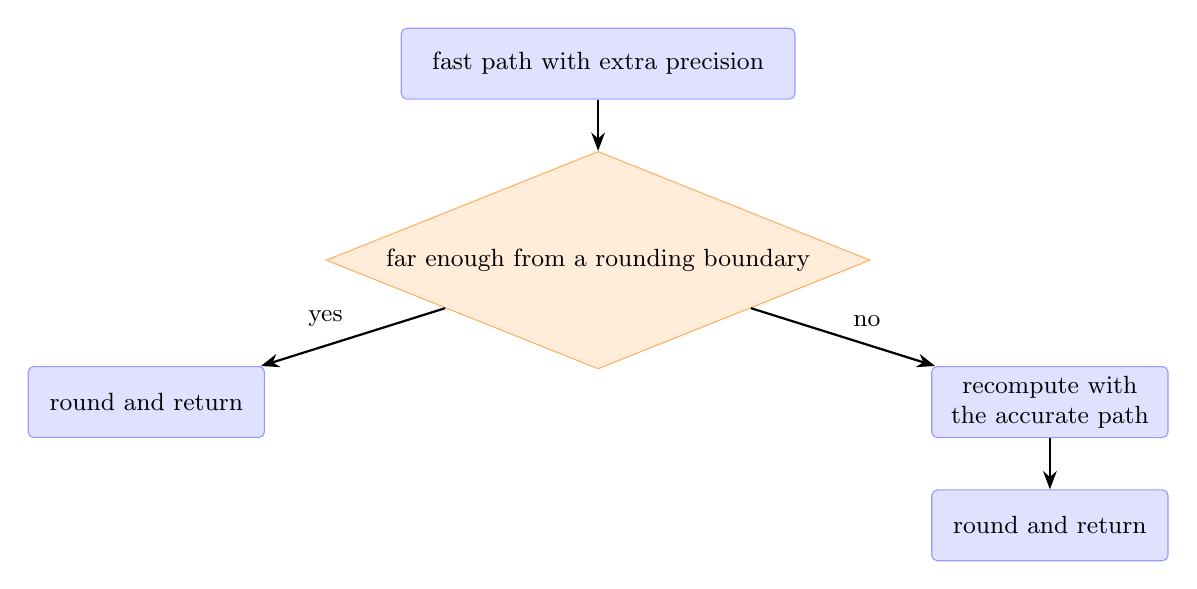
\begin{tikzpicture}[node distance=0.65cm and 2.5cm]
    \node (fast) [flowbox, minimum width=5cm] {fast path with extra precision};
    \node (dec)  [decisionbox, below=of fast] {far enough from a rounding boundary};
    \node (ret1) [flowbox, minimum width=3cm, below left=of dec]  {round and return};
    \node (acc)  [flowbox, minimum width=3cm, below right=of dec] {recompute with\\the accurate path};
    \node (ret2) [flowbox, minimum width=3cm, below=of acc]       {round and return};

    \draw[arrow] (fast) -- (dec);
    \draw[arrow] (dec) -- node[above left,  font=\small]{yes} (ret1);
    \draw[arrow] (dec) -- node[above right, font=\small]{no}  (acc);
    \draw[arrow] (acc) -- (ret2);
  \end{tikzpicture}
  \caption{Ziv's strategy as a fast-path test with a precise fallback.}
  \label{fig:ziv}
\end{figure}

Special cases are often where an implementation first reveals whether it was
designed from the contract or from the ordinary finite path.  The finite path
is only one part of the function.

% -----------------------------------------------------------------------
\section{CCMath rounding and standards policy}

CCMath functions should match the C++ math contract for the function being
implemented.  That includes finite values, special cases, overload behavior,
return type, NaNs, infinities, signed zeros, subnormals, overflow, underflow,
and rounding modes.

For floating-point math functions, the target is correct behavior under these
four IEEE rounding modes.

\begin{table}[h]
  \centering
  \begin{tabular}{ll}
    \toprule
    Mode & C \texttt{fenv} constant \\
    \midrule
    Round to nearest, ties to even & \texttt{FE\_TONEAREST} \\
    Round toward positive infinity  & \texttt{FE\_UPWARD} \\
    Round toward negative infinity  & \texttt{FE\_DOWNWARD} \\
    Round toward zero               & \texttt{FE\_TOWARDZERO} \\
    \bottomrule
  \end{tabular}
\end{table}

This affects dispatch.

A compiler builtin or platform libm call should not be assumed correct
outside round-to-nearest.  If a runtime path uses a builtin, SIMD
implementation, or platform function that is only known safe under
\texttt{FE\_TONEAREST}, the dispatcher must check the live rounding mode
first.

Directed modes should route to the generic kernel unless that fast path has
been proved and tested for the active mode.

The public header should not bypass that guard at runtime.  Constant
evaluation may use an eligible \texttt{constexpr} builtin when it satisfies
the same edge-case and accuracy policy.  Runtime calls should go through the
runtime dispatcher so the live rounding mode is observed.

This is part of the function contract.  A polynomial that works under
round-to-nearest is not automatically correct under \texttt{FE\_UPWARD},
\texttt{FE\_DOWNWARD}, or \texttt{FE\_TOWARDZERO}.  The final rounding step,
signed-zero cases, overflow thresholds, and underflow behavior may depend on
the active mode.

% -----------------------------------------------------------------------
\section{Tool roles}

\subsection{Sollya}

Use Sollya to bound approximation error for a stated function, interval,
error model, and coefficient format.  That step does not cover reduction,
evaluation, reconstruction, or final rounding.

\subsection{Gappa}

Use Gappa for floating-point error bounds in straight-line code.

This fits Horner kernels, Estrin kernels, compensated sums, split constants,
FMA sequences, and reconstruction fragments where the operation order is
fixed.

Sollya bounds the mathematical approximation error.  Gappa helps bound the
floating-point evaluation error.

\subsection{Rocq}

Rocq is an interactive theorem prover.

Use it when the proof needs a larger machine-checked structure: definitions,
lemmas, interval facts, rounding facts, and the link between local Gappa
proofs and the function-level theorem.

For CCMath, Rocq belongs to the high-assurance path, not the first pass for
every function.

\subsection{MPFR}

Use MPFR as the independent oracle.

MPFR testing is not a proof, but it is the usual way to validate an
implementation at scale.  Test random inputs, boundary inputs, subnormals,
overflow and underflow thresholds, exact cases, hard reduction cases, hard
rounding cases, and every supported rounding mode.

Measure ULP error.  Do not rely on printed decimal comparisons.

\subsection{SageMath}

Use SageMath for symbolic manipulation, series expansion, exact rational
arithmetic, continued fractions, interval experiments, and prototype
derivations.

For example, before writing a \texttt{log1p} kernel, inspect:
\[ \frac{\log(1+x)}{x} \]

Before writing a trig reducer, inspect continued-fraction approximants of
$\pi/2$.

SageMath is a scratch tool.  Sollya is the production coefficient path.

% -----------------------------------------------------------------------
\section{Checklist for a new function}

\subsection{Specify the target}

Write down the function, supported formats, supported rounding modes, domain,
special cases, accuracy target, and whether the goal is correct rounding,
faithful rounding, or a stated ULP bound.

Do this before writing the approximation.

\subsection{Choose the reduction}

Decide how the input maps into a small interval.

\begin{table}[h]
  \centering
  \begin{tabular}{ll}
    \toprule
    Function & Typical reduction \\
    \midrule
    $\exp(x)$   & $2^k$ times $\exp(r)$ \\
    $\log(x)$   & mantissa and exponent split \\
    trig        & reduction modulo $\pi/2$ or $\pi/4$ \\
    $\mathrm{pow}(x,y)$ & special integer paths, logarithmic paths, exact cases \\
    \bottomrule
  \end{tabular}
\end{table}

Also decide how much precision the reduction carries.

Record the sign, exponent, and significand split when the function uses it.

\subsection{Define the kernel}

Write the exact function that Sollya will approximate.

This may be $\sin(r)$, $\sin(r)/r$, $\exp(r)$, $\mathrm{expm1}(r)/r$,
$\log(1+r)/r$, a table residual, or another transformed function.

\subsection{Choose the interval}

Write the interval explicitly.
\begin{align*}
  r &\in \left[-\frac{\log 2}{2},\, \frac{\log 2}{2}\right] \\[4pt]
  r &\in \left[-\frac{\pi}{4},\, \frac{\pi}{4}\right]
\end{align*}

The approximation proof only holds on the interval that was checked.

\subsection{Choose the error model}

Choose absolute error, relative error, or a weighted error.

Use relative error when it matches ULP behavior.  Use absolute error or a
transformed kernel when relative error is ill-conditioned.

\subsection{Generate coefficients}

Use \texttt{guessdegree} to estimate the degree.  Then test nearby degrees.

Use \texttt{fpminimax} for production coefficients.

\begin{lstlisting}[style=sollya]
prec = 200!;
display = hexadecimal!;
\end{lstlisting}

Generate coefficients in the same formats used by the implementation.

\subsection{Generate the tables}

For each lookup table, record the invariant.

At minimum, write down the index formula, the represented real value, the
split format, the exactness constraint, the residual interval, and the
precision tier that consumes the table.

Generate separate tables for separate precision tiers when the split or
exactness constraint changes.

For log-style tables, record the residual formula, such as
$u = r_i(1 + m_x) - 1$, and the correction term supplied by the table.

\subsection{Check the approximation}

Use \texttt{dirtyinfnorm} for quick iteration.  Use \texttt{supnorm} for the
recorded bound.

Record the interval, polynomial degree, coefficient formats, error model,
and bound.

\subsection{Choose the evaluation scheme}

Choose Horner, Estrin, compensated Horner, double-word evaluation, or a
hybrid.

This choice is part of the proof.

\subsection{Choose the precision tiers}

Decide which inputs use the fast path and which inputs need an accurate path.

For float, double or double-double may be enough for many fast paths.

For double, expect a double-double-like fast path and a wider accurate path
for hard cases.

Use dyadic formats when the accurate path needs fixed precision and wider
exponent range.

\subsection{Prove the evaluation error}

Bound the floating-point error from the actual operation sequence.

Use Gappa where possible.  The approximation error alone is not enough.

Keep the total error budget visible.  The polynomial bound is only one term.

\subsection{Reconstruct and round}

Undo the reduction.  Handle scaling, quadrant selection, sign reconstruction,
table lookup, compensated addition, overflow, underflow, and double-rounding
hazards where they apply.

If the target is correct rounding, handle hard-to-round inputs or provide a
bounded strategy that covers them.

\subsection{Validate}

Compare against MPFR over random, structured, boundary, subnormal, overflow,
underflow, cancellation-heavy, and adversarial inputs.

Run every supported rounding mode.

\subsection{Record the status}

Document supported formats, supported rounding modes, maximum observed ULP,
proven bound if one exists, unsupported cases, known gaps, test coverage,
oracle used, and the relevant Sollya, Gappa, SageMath, or Rocq artifacts.

% -----------------------------------------------------------------------
\section{CCMath placement}

A typical function needs special-case handling, reduction constants,
approximation coefficients, an evaluation kernel, reconstruction logic,
rounding-mode handling, oracle tests, and status notes.

Generated constants are part of the algorithm.  If the interval, coefficient
format, polynomial degree, table split, or evaluation order changes, the
proof needs review.

Keep public APIs clean.  Put function-specific machinery in internal support
code.  Keep kernels small enough to audit.  Store or document enough
information to regenerate the constants.

If a function is only faithful, say so.  If only round-to-nearest has been
validated, say so.  If directed modes are not covered, say so.

Do not imply a stronger contract than the proof and tests support.

% -----------------------------------------------------------------------
\section{Other approaches}

\subsection{Traditional libm workflow}

The usual workflow matches Figure~\ref{fig:ziv}, with explicit bounds on
floating-point evaluation error before the final rounding argument.  Sollya
and Gappa fit this structure naturally.

\subsection{RLIBM-style result approximation}

RLIBM uses a different target~\cite{rlibm}.

The traditional route approximates the real function, then proves that
rounding gives the desired floating-point result.

RLIBM generates polynomials that target the correctly rounded floating-point
result directly.  The polynomial is trying to land inside the interval of
real values that round to the right floating-point answer.

Not the default CCMath workflow.  Worth studying for correctly rounded float
functions, generated libraries, and multi-format work.

\subsection{CRlibm and CORE-MATH}

CRlibm is useful for studying Ziv-test based correctly rounded
functions~\cite{crlibm,coremath}.

CORE-MATH is useful for modern correctly rounded elementary functions with
compact implementations and proof-oriented notes~\cite{coremath}.

Study the structure: reduction, approximation, reconstruction, hard cases,
proof.

% -----------------------------------------------------------------------
\section{Minimal Sollya template}

Start from the script in Section~9.  For a reproducible production script,
also print the certified bound and the coefficient forms:

\begin{lstlisting}[style=sollya]
eps_cert = supnorm(p, f, I, relative, 1b-40);
print("certified relative error:", eps_cert);

print("certified relative error bits:", log2(eps_cert));

print("canonical:");
canonical(p);

print("horner:");
horner(p);
\end{lstlisting}

Keep the script with the implementation or proof tooling.  Constants in
source should be reproducible from the script.

% -----------------------------------------------------------------------
\section{Minimal SageMath scratch template}

Use SageMath before the production Sollya script when the algebra is still
being explored.

\begin{lstlisting}[style=shell]
var('x')

f = log(1 + x) / x
series(f, x, 0, 10)
\end{lstlisting}

For continued fractions:
\begin{lstlisting}[style=shell]
continued_fraction(pi / 2).convergents()[:10]
\end{lstlisting}

For exact rational checks:
\begin{lstlisting}[style=shell]
R = RationalField()
a = R(355) / R(113)
a - pi.n(100)
\end{lstlisting}

Treat these as exploration unless the exact claim is recorded and checked as
part of the proof.

% -----------------------------------------------------------------------
\section{Citation policy}

Citations use ACM numeric style with \texttt{ACM-Reference-Format.bst}.
Prefer full author names and stable DOI or URL fields in the bibliography.

\begin{table}[h]
  \centering
  \begin{tabular}{p{4.5cm}p{7cm}}
    \toprule
    Source & Typical use in this guide \\
    \midrule
    IEEE 754-2019~\cite{ieee}
      & Required operations, rounding modes, exceptions, NaNs, infinities,
        signed zeros, subnormals \\
    Muller, \emph{Elementary Functions}~\cite{muller}
      & Minimax approximation, Remez, range reduction, Cody-Waite,
        Payne-Hanek, Ziv tests \\
    \emph{Handbook of Floating-Point Arithmetic}~\cite{handbook}
      & ULPs, FMA, double-word arithmetic, compiler hazards, Gappa, MPFR \\
    Sollya~\cite{sollya}
      & Command syntax and coefficient generation \\
    Gappa~\cite{gappa}
      & Straight-line floating-point error proofs \\
    Rocq~\cite{rocq}
      & Machine-checked proof structure \\
    SageMath~\cite{sagemath}
      & Symbolic exploration before production scripts \\
    MPFR~\cite{mpfr}
      & Oracle reference behavior \\
    RLIBM~\cite{rlibm}
      & Direct approximation of the correctly rounded result \\
    Goldberg~\cite{goldberg}, Oracle NCG~\cite{oracle}
      & Introductory floating-point background \\
    \bottomrule
  \end{tabular}
\end{table}

% -----------------------------------------------------------------------
\section{Further reading}

Free resources come first.  Paid books follow for deeper derivations and
citable design notes.  Each entry lists a URL and what it covers.

\subsection{Free resources}

\subsubsection{First pass on floating point.}

\emph{Oracle reprint of Goldberg, What Every Computer Scientist Should Know
About Floating-Point Arithmetic.}
\url{https://docs.oracle.com/cd/E19957-01/806-3568/ncg_goldberg.html}\\
Introductory floating-point article.  Covers rounding, guard digits,
cancellation, ULPs, and IEEE arithmetic.

\emph{The Floating-Point Guide.}
\url{https://floating-point-gui.de/}\\
Short beginner reference on binary floating-point behavior, not libm design.

\emph{IEEE~754-2019 official page.}
\url{https://standards.ieee.org/standard/754-2019.html}\\
Official standard page.  The full text is not free on every access path.

\subsubsection{Sollya and approximation work.}

\emph{Sollya official site.}
\url{https://www.sollya.org/}\\
Tool site and current manual.  Minimax approximation, constrained
coefficients, and certified supremum-norm checks.

\emph{Sollya \texttt{fpminimax} documentation.}
\url{https://www.sollya.org/sollya-current/help.php?name=fpminimax}\\
Command reference for production coefficients in requested floating-point
formats.

\emph{Sollya \texttt{supnorm} documentation.}
\url{https://www.sollya.org/sollya-current/help.php?name=supnorm}\\
Recorded approximation bounds.  Run after quick \texttt{dirtyinfnorm} checks.

\subsubsection{Proof and validation tools.}

\emph{Gappa user guide.}
\url{https://gappa.gitlabpages.inria.fr/gappa/index.html}\\
Straight-line floating-point and fixed-point error proofs after Sollya.

\emph{Rocq Prover reference manual.}
\url{https://rocq-prover.org/refman}\\
Machine-checked proof structure beyond local Gappa bounds.

\emph{GNU MPFR official site.}
\url{https://www.mpfr.org/}\\
High-precision oracle with correct rounding.

\emph{SageMath documentation.}
\url{https://doc.sagemath.org/}\\
Symbolic exploration before production Sollya scripts: series, exact
rationals, and continued fractions.

\subsubsection{Implementations and current research.}

\emph{LLVM libc math status.}
\url{https://libc.llvm.org/math/}\\
LLVM libc math accuracy table, including functions marked correctly rounded
in all four rounding modes.

\emph{CORE-MATH project.}
\url{https://core-math.gitlabpages.inria.fr/}\\
Compact correctly rounded implementations and proof-oriented notes.

\emph{CORE-MATH paper.}
\url{https://inria.hal.science/hal-03721525v3/file/core-math-final.pdf}\\
Project goals and design direction.

\emph{RLIBM project page.}
\url{https://people.cs.rutgers.edu/~sn349/rlibm/}\\
Polynomials that target the correctly rounded floating-point result directly.

\emph{RLIBM-ALL paper.}
\url{https://arxiv.org/abs/2108.06756}\\
Multi-format, multi-rounding-mode RLIBM.

\emph{RLIBM-MultiRound paper.}
\url{https://arxiv.org/abs/2504.07409}\\
Rounding-mode switching cost and methods that avoid depending on the live
mode.

\emph{CRlibm report.}
\url{https://ens-lyon.hal.science/ensl-01529804v1/document}\\
Correctly rounded elementary functions and Ziv-style design.

\subsubsection{Performance-oriented implementation references.}

\emph{SLEEF paper.}
\url{https://www.shibatch.net/sleef/}\\
Portable vectorized elementary functions with explicit vector paths and
accuracy targets~\cite{sleef}.

\emph{LLVM libc math slides.}
\url{https://libc.llvm.org/math/}\\
Modern CPU instructions, FMA, and rounding instructions in LLVM libc math
work.

\emph{Arm Optimized Routines.}
\url{https://www.arm.com/why-arm/technologies/compute-library}\\
Target-specific scalar and vector math routines for Arm CPUs~\cite{arm}.

\emph{Agner Fog optimization manuals.}
\url{https://www.agner.org/optimize/}\\
CPU microarchitecture, instruction timing, and low-level performance
notes~\cite{fog}.

\emph{Intel optimization manual.}
\url{https://www.intel.com/content/www/us/en/developer/articles/technical/intel-sdm.html}\\
Intel x86 tuning and instruction behavior~\cite{intel}.

\emph{AMD Zen optimization guide.}
\url{https://developer.amd.com/resources/developer-guides-manuals/}\\
AMD-specific tuning for Zen-family processors~\cite{amd}.

\subsubsection{Survey and background papers.}

\emph{Floating-point arithmetic, Acta Numerica survey.}
\url{https://www.cambridge.org/core/journals/acta-numerica/article/floating-point-arithmetic/287C4D5F6D4A43FBEEB1ABED2A405AAF}\\
Modern survey of floating-point arithmetic and IEEE behavior.

\emph{Gappa paper, Certification of bounds on expressions involving rounded
operators.}
\url{https://arxiv.org/abs/cs/0701186}\\
Paper behind the Gappa tool.

\emph{MPFR paper, A Multiple-Precision Binary Floating-Point Library with
Correct Rounding.}
\url{https://inria.hal.science/inria-00070266v1/document}\\
Design of the usual high-precision oracle.

\subsection{Paid books and standards}

\subsubsection{Best main book for elementary functions.}

\emph{Elementary Functions: Algorithms and Implementation}, Jean-Michel
Muller, Springer.
\url{https://link.springer.com/book/10.1007/978-1-4899-7983-4}\\
Exp, log, trig functions, range reduction, polynomial approximation, table
methods, and correct rounding.

\subsubsection{Best main book for floating-point arithmetic.}

\emph{Handbook of Floating-Point Arithmetic}, 2nd edition, Springer.
\url{https://link.springer.com/book/10.1007/978-3-319-76526-6}\\
Floating-point formats, rounding, ULPs, FMA, exceptions, compiler issues,
Gappa, MPFR, and formal verification.

\subsubsection{Strong general book on finite precision error.}

\emph{Accuracy and Stability of Numerical Algorithms}, Nicholas J. Higham,
SIAM.
\url{https://epubs.siam.org/doi/10.1137/1.9780898718027}\\
Numerical error, stability, and finite precision analysis, not libm design.

\subsubsection{Shorter IEEE floating-point book.}

\emph{Numerical Computing with IEEE Floating Point Arithmetic}, Michael L.
Overton, SIAM.
\url{https://epubs.siam.org/doi/book/10.1137/1.9780898718072}\\
Shorter IEEE floating-point introduction than the Handbook.

\subsubsection{Historical libm implementation reference.}

\emph{Software Manual for the Elementary Functions}, Cody and Waite.
\url{https://www.amazon.com/Elementary-Functions-Prentice-Hall-computational-mathematics/dp/0138220646}\\
Classic libm structure: reduction, rational approximation, special cases, and
implementation constants.  Not a modern correctness target.

\subsubsection{Official floating-point standard.}

\emph{IEEE 754-2019 official standard page.}
\url{https://standards.ieee.org/standard/754-2019.html}\\
Authoritative standard for floating-point formats, rounding attributes,
exceptions, NaNs, infinities, signed zeros, subnormals, and required
operations.

% -----------------------------------------------------------------------
\bibliographystyle{ACM-Reference-Format}
\bibliography{approx_functions}

% -----------------------------------------------------------------------
\appendix

\section{Useful vocabulary}

\begin{table}[h]
  \centering
  \begin{tabular}{p{3.8cm}p{8.5cm}}
    \toprule
    Term & Meaning \\
    \midrule
    argument reduction
      & A mapping from the public input to a smaller interval where
        approximation is easier. \\
    kernel
      & The exact function that is actually approximated after reduction. \\
    transformed kernel
      & A kernel rewritten to remove a zero, cancellation point, or unstable
        relative error. \\
    reduced interval
      & The interval on which the approximation bound is claimed. \\
    residual
      & The small quantity that remains after a table lookup or other
        reduction step. \\
    reconstruction
      & The step that combines the reduced result with exponents, table
        constants, signs, or quadrants. \\
    minimax polynomial
      & A polynomial that minimizes the worst error on a stated interval. \\
    coefficient format
      & The floating-point or fixed-width format in which the implementation
        stores the coefficients. \\
    evaluation scheme
      & The operation order used to evaluate the polynomial, such as Horner
        or Estrin. \\
    table invariant
      & The exact real relation that a table entry is meant to support. \\
    exactness constraint
      & A requirement that one later operation be exact or tightly bounded
        because of how a constant was split. \\
    faithful rounding
      & Returning one of the two floating-point neighbors of the exact
        result. \\
    correct rounding
      & Returning the value selected by the active rounding mode from the
        exact real result. \\
    hard case
      & An input whose exact result lies unusually close to a rounding
        boundary. \\
    oracle
      & An independent high-precision reference used for validation, usually
        MPFR in this workflow. \\
    fast path
      & The cheap path intended for ordinary inputs. \\
    accurate path
      & The slower path used when the fast path cannot justify the final
        rounding decision. \\
    ULP
      & The gap between consecutive floating-point values at a given
        magnitude. \\
    \bottomrule
  \end{tabular}
\end{table}

% -----------------------------------------------------------------------
\section{How the proof pieces fit together}

Keep these obligations separate when reading or writing a proof note.

\begin{enumerate}
\item \textbf{Reduction bound:} distance between the computed reduced
  argument and the exact reduced argument.
\item \textbf{Approximation bound:} distance between the mathematical
  polynomial and the kernel on the reduced interval.
\item \textbf{Evaluation bound:} rounding error from the compiled operation
  sequence that evaluates the polynomial.
\item \textbf{Reconstruction bound:} effect of split constants, exponent
  additions, sign fixes, and table lookups.
\item \textbf{Rounding argument:} margin to a rounding boundary, or the need
  for a fallback path.
\item \textbf{Oracle validation:} agreement with an independent reference
  over many inputs.  Engineering evidence, not a proof certificate.
\end{enumerate}

A small approximation error does not fix a bad reduction.  A split table does
not prove the polynomial.  MPFR agreement does not certify the floating-point
circuit.  State which obligation each artifact covers.

\end{document}
